% !TEX encoding = UTF-8 Unicode
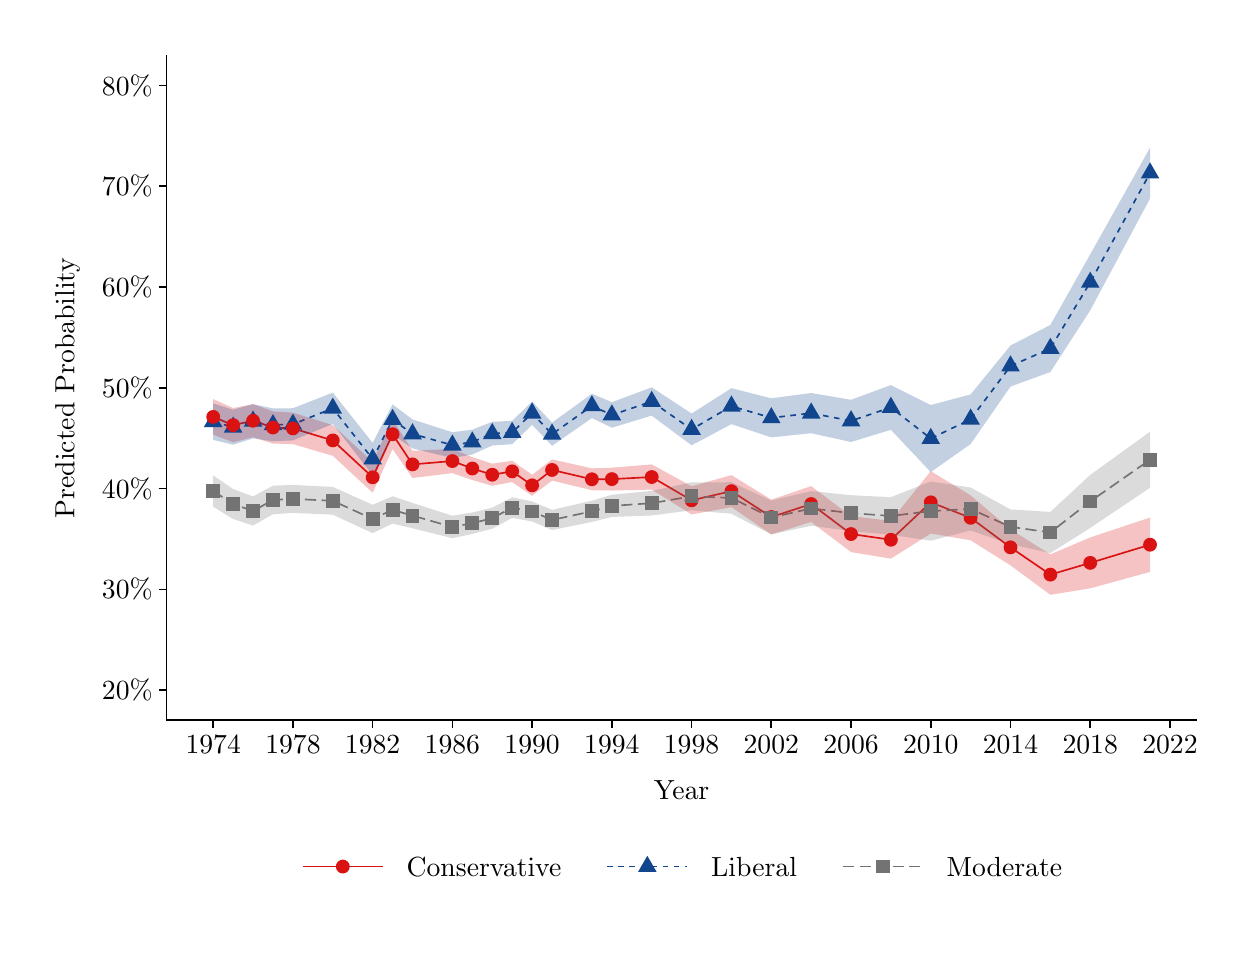
\begin{tikzpicture}[x=1pt,y=1pt]
\definecolor{fillColor}{RGB}{255,255,255}
\path[use as bounding box,fill=fillColor,fill opacity=0.00] (0,0) rectangle (432.48,324.36);
\begin{scope}
\path[clip] (  0.00,  0.00) rectangle (432.48,324.36);
\definecolor{fillColor}{RGB}{255,255,255}

\path[fill=fillColor] ( -0.00,  0.00) rectangle (432.48,324.36);
\end{scope}
\begin{scope}
\path[clip] ( 50.11, 74.07) rectangle (422.48,314.36);
\definecolor{fillColor}{RGB}{255,255,255}

\path[fill=fillColor] ( 50.11, 74.07) rectangle (422.48,314.36);
\definecolor{drawColor}{RGB}{218,18,18}

\path[draw=drawColor,line width= 0.6pt,line join=round] ( 67.04,183.71) --
	( 74.24,180.73) --
	( 81.44,182.33) --
	( 88.64,179.88) --
	( 95.85,179.55) --
	(110.25,175.21) --
	(124.66,161.89) --
	(131.86,177.45) --
	(139.06,166.55) --
	(153.47,167.76) --
	(160.67,165.05) --
	(167.87,162.81) --
	(175.07,164.03) --
	(182.28,158.98) --
	(189.48,164.54) --
	(203.88,161.17) --
	(211.09,161.23) --
	(225.49,161.98) --
	(239.90,153.56) --
	(254.30,156.88) --
	(268.71,147.53) --
	(283.11,152.22) --
	(297.52,141.38) --
	(311.92,139.32) --
	(326.33,152.84) --
	(340.73,147.24) --
	(355.14,136.57) --
	(369.54,126.72) --
	(383.95,130.96) --
	(405.56,137.53);
\definecolor{drawColor}{RGB}{17,70,143}

\path[draw=drawColor,line width= 0.6pt,dash pattern=on 2pt off 2pt ,line join=round] ( 67.04,181.98) --
	( 74.24,179.99) --
	( 81.44,182.14) --
	( 88.64,180.84) --
	( 95.85,181.03) --
	(110.25,186.83) --
	(124.66,168.51) --
	(131.86,182.76) --
	(139.06,177.56) --
	(153.47,173.50) --
	(160.67,174.61) --
	(167.87,177.66) --
	(175.07,178.07) --
	(182.28,185.06) --
	(189.48,177.45) --
	(203.88,187.70) --
	(211.09,184.40) --
	(225.49,189.28) --
	(239.90,179.18) --
	(254.30,187.59) --
	(268.71,183.37) --
	(283.11,185.07) --
	(297.52,182.27) --
	(311.92,187.13) --
	(326.33,175.88) --
	(340.73,182.86) --
	(355.14,202.09) --
	(369.54,208.43) --
	(383.95,232.33) --
	(405.56,271.80);
\definecolor{drawColor}{gray}{0.45}

\path[draw=drawColor,line width= 0.6pt,dash pattern=on 4pt off 2pt ,line join=round] ( 67.04,156.91) --
	( 74.24,152.22) --
	( 81.44,149.72) --
	( 88.64,153.69) --
	( 95.85,154.08) --
	(110.25,153.39) --
	(124.66,146.83) --
	(131.86,150.10) --
	(139.06,148.04) --
	(153.47,143.94) --
	(160.67,145.29) --
	(167.87,147.10) --
	(175.07,150.93) --
	(182.28,149.55) --
	(189.48,146.48) --
	(203.88,149.59) --
	(211.09,151.55) --
	(225.49,152.53) --
	(239.90,155.01) --
	(254.30,154.41) --
	(268.71,147.36) --
	(283.11,150.63) --
	(297.52,148.95) --
	(311.92,147.91) --
	(326.33,149.67) --
	(340.73,150.44) --
	(355.14,143.98) --
	(369.54,141.95) --
	(383.95,153.17) --
	(405.56,168.24);
\definecolor{fillColor}{RGB}{218,18,18}

\path[fill=fillColor,fill opacity=0.25] ( 67.04,190.13) --
	( 74.24,186.90) --
	( 81.44,188.32) --
	( 88.64,185.70) --
	( 95.85,185.23) --
	(110.25,180.75) --
	(124.66,167.44) --
	(131.86,182.79) --
	(139.06,171.47) --
	(153.47,172.13) --
	(160.67,169.18) --
	(167.87,166.79) --
	(175.07,167.88) --
	(182.28,162.76) --
	(189.48,168.36) --
	(203.88,165.12) --
	(211.09,165.35) --
	(225.49,166.54) --
	(239.90,158.64) --
	(254.30,162.67) --
	(268.71,153.80) --
	(283.11,158.69) --
	(297.52,147.89) --
	(311.92,146.14) --
	(326.33,164.11) --
	(340.73,155.35) --
	(355.14,143.07) --
	(369.54,134.02) --
	(383.95,140.14) --
	(405.56,147.35) --
	(405.56,127.70) --
	(383.95,121.77) --
	(369.54,119.43) --
	(355.14,130.07) --
	(340.73,139.13) --
	(326.33,141.57) --
	(311.92,132.50) --
	(297.52,134.86) --
	(283.11,145.76) --
	(268.71,141.25) --
	(254.30,151.09) --
	(239.90,148.47) --
	(225.49,157.43) --
	(211.09,157.11) --
	(203.88,157.21) --
	(189.48,160.71) --
	(182.28,155.20) --
	(175.07,160.17) --
	(167.87,158.82) --
	(160.67,160.91) --
	(153.47,163.40) --
	(139.06,161.63) --
	(131.86,172.11) --
	(124.66,156.33) --
	(110.25,169.67) --
	( 95.85,173.87) --
	( 88.64,174.07) --
	( 81.44,176.34) --
	( 74.24,174.55) --
	( 67.04,177.30) --
	cycle;

\path[] ( 67.04,190.13) --
	( 74.24,186.90) --
	( 81.44,188.32) --
	( 88.64,185.70) --
	( 95.85,185.23) --
	(110.25,180.75) --
	(124.66,167.44) --
	(131.86,182.79) --
	(139.06,171.47) --
	(153.47,172.13) --
	(160.67,169.18) --
	(167.87,166.79) --
	(175.07,167.88) --
	(182.28,162.76) --
	(189.48,168.36) --
	(203.88,165.12) --
	(211.09,165.35) --
	(225.49,166.54) --
	(239.90,158.64) --
	(254.30,162.67) --
	(268.71,153.80) --
	(283.11,158.69) --
	(297.52,147.89) --
	(311.92,146.14) --
	(326.33,164.11) --
	(340.73,155.35) --
	(355.14,143.07) --
	(369.54,134.02) --
	(383.95,140.14) --
	(405.56,147.35);

\path[] (405.56,127.70) --
	(383.95,121.77) --
	(369.54,119.43) --
	(355.14,130.07) --
	(340.73,139.13) --
	(326.33,141.57) --
	(311.92,132.50) --
	(297.52,134.86) --
	(283.11,145.76) --
	(268.71,141.25) --
	(254.30,151.09) --
	(239.90,148.47) --
	(225.49,157.43) --
	(211.09,157.11) --
	(203.88,157.21) --
	(189.48,160.71) --
	(182.28,155.20) --
	(175.07,160.17) --
	(167.87,158.82) --
	(160.67,160.91) --
	(153.47,163.40) --
	(139.06,161.63) --
	(131.86,172.11) --
	(124.66,156.33) --
	(110.25,169.67) --
	( 95.85,173.87) --
	( 88.64,174.07) --
	( 81.44,176.34) --
	( 74.24,174.55) --
	( 67.04,177.30);
\definecolor{fillColor}{RGB}{17,70,143}

\path[fill=fillColor,fill opacity=0.25] ( 67.04,188.57) --
	( 74.24,186.31) --
	( 81.44,188.32) --
	( 88.64,186.79) --
	( 95.85,186.84) --
	(110.25,192.47) --
	(124.66,174.34) --
	(131.86,188.22) --
	(139.06,182.79) --
	(153.47,178.17) --
	(160.67,179.09) --
	(167.87,181.94) --
	(175.07,182.28) --
	(182.28,189.29) --
	(189.48,181.62) --
	(203.88,192.10) --
	(211.09,189.00) --
	(225.49,194.39) --
	(239.90,184.91) --
	(254.30,194.08) --
	(268.71,190.43) --
	(283.11,192.34) --
	(297.52,189.89) --
	(311.92,195.21) --
	(326.33,187.99) --
	(340.73,191.82) --
	(355.14,209.51) --
	(369.54,216.92) --
	(383.95,242.44) --
	(405.56,280.98) --
	(405.56,262.62) --
	(383.95,222.21) --
	(369.54,199.94) --
	(355.14,194.67) --
	(340.73,173.91) --
	(326.33,163.77) --
	(311.92,179.05) --
	(297.52,174.64) --
	(283.11,177.81) --
	(268.71,176.32) --
	(254.30,181.09) --
	(239.90,173.45) --
	(225.49,184.18) --
	(211.09,179.80) --
	(203.88,183.29) --
	(189.48,173.28) --
	(182.28,180.84) --
	(175.07,173.85) --
	(167.87,173.38) --
	(160.67,170.14) --
	(153.47,168.84) --
	(139.06,172.32) --
	(131.86,177.30) --
	(124.66,162.67) --
	(110.25,181.19) --
	( 95.85,175.22) --
	( 88.64,174.89) --
	( 81.44,175.97) --
	( 74.24,173.67) --
	( 67.04,175.39) --
	cycle;

\path[] ( 67.04,188.57) --
	( 74.24,186.31) --
	( 81.44,188.32) --
	( 88.64,186.79) --
	( 95.85,186.84) --
	(110.25,192.47) --
	(124.66,174.34) --
	(131.86,188.22) --
	(139.06,182.79) --
	(153.47,178.17) --
	(160.67,179.09) --
	(167.87,181.94) --
	(175.07,182.28) --
	(182.28,189.29) --
	(189.48,181.62) --
	(203.88,192.10) --
	(211.09,189.00) --
	(225.49,194.39) --
	(239.90,184.91) --
	(254.30,194.08) --
	(268.71,190.43) --
	(283.11,192.34) --
	(297.52,189.89) --
	(311.92,195.21) --
	(326.33,187.99) --
	(340.73,191.82) --
	(355.14,209.51) --
	(369.54,216.92) --
	(383.95,242.44) --
	(405.56,280.98);

\path[] (405.56,262.62) --
	(383.95,222.21) --
	(369.54,199.94) --
	(355.14,194.67) --
	(340.73,173.91) --
	(326.33,163.77) --
	(311.92,179.05) --
	(297.52,174.64) --
	(283.11,177.81) --
	(268.71,176.32) --
	(254.30,181.09) --
	(239.90,173.45) --
	(225.49,184.18) --
	(211.09,179.80) --
	(203.88,183.29) --
	(189.48,173.28) --
	(182.28,180.84) --
	(175.07,173.85) --
	(167.87,173.38) --
	(160.67,170.14) --
	(153.47,168.84) --
	(139.06,172.32) --
	(131.86,177.30) --
	(124.66,162.67) --
	(110.25,181.19) --
	( 95.85,175.22) --
	( 88.64,174.89) --
	( 81.44,175.97) --
	( 74.24,173.67) --
	( 67.04,175.39);
\definecolor{fillColor}{RGB}{115,115,115}

\path[fill=fillColor,fill opacity=0.25] ( 67.04,162.56) --
	( 74.24,157.63) --
	( 81.44,154.97) --
	( 88.64,158.84) --
	( 95.85,159.13) --
	(110.25,158.40) --
	(124.66,151.96) --
	(131.86,155.03) --
	(139.06,152.61) --
	(153.47,148.00) --
	(160.67,149.17) --
	(167.87,150.91) --
	(175.07,154.64) --
	(182.28,153.16) --
	(189.48,150.12) --
	(203.88,153.43) --
	(211.09,155.56) --
	(225.49,156.97) --
	(239.90,160.07) --
	(254.30,160.10) --
	(268.71,153.47) --
	(283.11,156.90) --
	(297.52,155.41) --
	(311.92,154.70) --
	(326.33,160.38) --
	(340.73,158.18) --
	(355.14,150.27) --
	(369.54,149.38) --
	(383.95,162.74) --
	(405.56,178.35) --
	(405.56,158.12) --
	(383.95,143.59) --
	(369.54,134.52) --
	(355.14,137.68) --
	(340.73,142.69) --
	(326.33,138.97) --
	(311.92,141.12) --
	(297.52,142.48) --
	(283.11,144.36) --
	(268.71,141.25) --
	(254.30,148.72) --
	(239.90,149.96) --
	(225.49,148.09) --
	(211.09,147.55) --
	(203.88,145.76) --
	(189.48,142.83) --
	(182.28,145.93) --
	(175.07,147.22) --
	(167.87,143.29) --
	(160.67,141.42) --
	(153.47,139.88) --
	(139.06,143.47) --
	(131.86,145.17) --
	(124.66,141.71) --
	(110.25,148.38) --
	( 95.85,149.02) --
	( 88.64,148.54) --
	( 81.44,144.47) --
	( 74.24,146.82) --
	( 67.04,151.26) --
	cycle;

\path[] ( 67.04,162.56) --
	( 74.24,157.63) --
	( 81.44,154.97) --
	( 88.64,158.84) --
	( 95.85,159.13) --
	(110.25,158.40) --
	(124.66,151.96) --
	(131.86,155.03) --
	(139.06,152.61) --
	(153.47,148.00) --
	(160.67,149.17) --
	(167.87,150.91) --
	(175.07,154.64) --
	(182.28,153.16) --
	(189.48,150.12) --
	(203.88,153.43) --
	(211.09,155.56) --
	(225.49,156.97) --
	(239.90,160.07) --
	(254.30,160.10) --
	(268.71,153.47) --
	(283.11,156.90) --
	(297.52,155.41) --
	(311.92,154.70) --
	(326.33,160.38) --
	(340.73,158.18) --
	(355.14,150.27) --
	(369.54,149.38) --
	(383.95,162.74) --
	(405.56,178.35);

\path[] (405.56,158.12) --
	(383.95,143.59) --
	(369.54,134.52) --
	(355.14,137.68) --
	(340.73,142.69) --
	(326.33,138.97) --
	(311.92,141.12) --
	(297.52,142.48) --
	(283.11,144.36) --
	(268.71,141.25) --
	(254.30,148.72) --
	(239.90,149.96) --
	(225.49,148.09) --
	(211.09,147.55) --
	(203.88,145.76) --
	(189.48,142.83) --
	(182.28,145.93) --
	(175.07,147.22) --
	(167.87,143.29) --
	(160.67,141.42) --
	(153.47,139.88) --
	(139.06,143.47) --
	(131.86,145.17) --
	(124.66,141.71) --
	(110.25,148.38) --
	( 95.85,149.02) --
	( 88.64,148.54) --
	( 81.44,144.47) --
	( 74.24,146.82) --
	( 67.04,151.26);
\definecolor{fillColor}{RGB}{17,70,143}

\path[fill=fillColor] ( 67.04,185.86) --
	( 70.40,180.04) --
	( 63.67,180.04) --
	cycle;

\path[fill=fillColor] ( 74.24,183.88) --
	( 77.60,178.05) --
	( 70.87,178.05) --
	cycle;

\path[fill=fillColor] ( 81.44,186.03) --
	( 84.80,180.20) --
	( 78.08,180.20) --
	cycle;

\path[fill=fillColor] ( 88.64,184.72) --
	( 92.01,178.90) --
	( 85.28,178.90) --
	cycle;

\path[fill=fillColor] ( 95.85,184.91) --
	( 99.21,179.09) --
	( 92.48,179.09) --
	cycle;

\path[fill=fillColor] (110.25,190.71) --
	(113.62,184.89) --
	(106.89,184.89) --
	cycle;

\path[fill=fillColor] (124.66,172.39) --
	(128.02,166.56) --
	(121.29,166.56) --
	cycle;

\path[fill=fillColor] (131.86,186.65) --
	(135.22,180.82) --
	(128.50,180.82) --
	cycle;

\path[fill=fillColor] (139.06,181.44) --
	(142.43,175.61) --
	(135.70,175.61) --
	cycle;

\path[fill=fillColor] (153.47,177.39) --
	(156.83,171.56) --
	(150.10,171.56) --
	cycle;

\path[fill=fillColor] (160.67,178.50) --
	(164.03,172.67) --
	(157.31,172.67) --
	cycle;

\path[fill=fillColor] (167.87,181.55) --
	(171.24,175.72) --
	(164.51,175.72) --
	cycle;

\path[fill=fillColor] (175.07,181.95) --
	(178.44,176.13) --
	(171.71,176.13) --
	cycle;

\path[fill=fillColor] (182.28,188.95) --
	(185.64,183.12) --
	(178.91,183.12) --
	cycle;

\path[fill=fillColor] (189.48,181.34) --
	(192.84,175.51) --
	(186.12,175.51) --
	cycle;

\path[fill=fillColor] (203.88,191.58) --
	(207.25,185.76) --
	(200.52,185.76) --
	cycle;

\path[fill=fillColor] (211.09,188.28) --
	(214.45,182.46) --
	(207.72,182.46) --
	cycle;

\path[fill=fillColor] (225.49,193.17) --
	(228.86,187.34) --
	(222.13,187.34) --
	cycle;

\path[fill=fillColor] (239.90,183.06) --
	(243.26,177.24) --
	(236.53,177.24) --
	cycle;

\path[fill=fillColor] (254.30,191.47) --
	(257.67,185.64) --
	(250.94,185.64) --
	cycle;

\path[fill=fillColor] (268.71,187.26) --
	(272.07,181.43) --
	(265.34,181.43) --
	cycle;

\path[fill=fillColor] (283.11,188.96) --
	(286.48,183.13) --
	(279.75,183.13) --
	cycle;

\path[fill=fillColor] (297.52,186.15) --
	(300.88,180.33) --
	(294.15,180.33) --
	cycle;

\path[fill=fillColor] (311.92,191.01) --
	(315.29,185.19) --
	(308.56,185.19) --
	cycle;

\path[fill=fillColor] (326.33,179.77) --
	(329.69,173.94) --
	(322.96,173.94) --
	cycle;

\path[fill=fillColor] (340.73,186.75) --
	(344.10,180.92) --
	(337.37,180.92) --
	cycle;

\path[fill=fillColor] (355.14,205.97) --
	(358.50,200.15) --
	(351.77,200.15) --
	cycle;

\path[fill=fillColor] (369.54,212.31) --
	(372.91,206.49) --
	(366.18,206.49) --
	cycle;

\path[fill=fillColor] (383.95,236.21) --
	(387.31,230.39) --
	(380.58,230.39) --
	cycle;

\path[fill=fillColor] (405.56,275.69) --
	(408.92,269.86) --
	(402.19,269.86) --
	cycle;
\definecolor{fillColor}{RGB}{218,18,18}

\path[fill=fillColor] ( 67.04,183.71) circle (  2.50);

\path[fill=fillColor] ( 74.24,180.73) circle (  2.50);

\path[fill=fillColor] ( 81.44,182.33) circle (  2.50);

\path[fill=fillColor] ( 88.64,179.88) circle (  2.50);

\path[fill=fillColor] ( 95.85,179.55) circle (  2.50);

\path[fill=fillColor] (110.25,175.21) circle (  2.50);

\path[fill=fillColor] (124.66,161.89) circle (  2.50);

\path[fill=fillColor] (131.86,177.45) circle (  2.50);

\path[fill=fillColor] (139.06,166.55) circle (  2.50);

\path[fill=fillColor] (153.47,167.76) circle (  2.50);

\path[fill=fillColor] (160.67,165.05) circle (  2.50);

\path[fill=fillColor] (167.87,162.81) circle (  2.50);

\path[fill=fillColor] (175.07,164.03) circle (  2.50);

\path[fill=fillColor] (182.28,158.98) circle (  2.50);

\path[fill=fillColor] (189.48,164.54) circle (  2.50);

\path[fill=fillColor] (203.88,161.17) circle (  2.50);

\path[fill=fillColor] (211.09,161.23) circle (  2.50);

\path[fill=fillColor] (225.49,161.98) circle (  2.50);

\path[fill=fillColor] (239.90,153.56) circle (  2.50);

\path[fill=fillColor] (254.30,156.88) circle (  2.50);

\path[fill=fillColor] (268.71,147.53) circle (  2.50);

\path[fill=fillColor] (283.11,152.22) circle (  2.50);

\path[fill=fillColor] (297.52,141.38) circle (  2.50);

\path[fill=fillColor] (311.92,139.32) circle (  2.50);

\path[fill=fillColor] (326.33,152.84) circle (  2.50);

\path[fill=fillColor] (340.73,147.24) circle (  2.50);

\path[fill=fillColor] (355.14,136.57) circle (  2.50);

\path[fill=fillColor] (369.54,126.72) circle (  2.50);

\path[fill=fillColor] (383.95,130.96) circle (  2.50);

\path[fill=fillColor] (405.56,137.53) circle (  2.50);
\definecolor{fillColor}{gray}{0.45}

\path[fill=fillColor] ( 64.54,154.41) --
	( 69.53,154.41) --
	( 69.53,159.41) --
	( 64.54,159.41) --
	cycle;

\path[fill=fillColor] ( 71.74,149.72) --
	( 76.74,149.72) --
	( 76.74,154.72) --
	( 71.74,154.72) --
	cycle;

\path[fill=fillColor] ( 78.94,147.22) --
	( 83.94,147.22) --
	( 83.94,152.22) --
	( 78.94,152.22) --
	cycle;

\path[fill=fillColor] ( 86.15,151.20) --
	( 91.14,151.20) --
	( 91.14,156.19) --
	( 86.15,156.19) --
	cycle;

\path[fill=fillColor] ( 93.35,151.58) --
	( 98.34,151.58) --
	( 98.34,156.57) --
	( 93.35,156.57) --
	cycle;

\path[fill=fillColor] (107.75,150.89) --
	(112.75,150.89) --
	(112.75,155.89) --
	(107.75,155.89) --
	cycle;

\path[fill=fillColor] (122.16,144.34) --
	(127.15,144.34) --
	(127.15,149.33) --
	(122.16,149.33) --
	cycle;

\path[fill=fillColor] (129.36,147.60) --
	(134.36,147.60) --
	(134.36,152.59) --
	(129.36,152.59) --
	cycle;

\path[fill=fillColor] (136.56,145.54) --
	(141.56,145.54) --
	(141.56,150.54) --
	(136.56,150.54) --
	cycle;

\path[fill=fillColor] (150.97,141.44) --
	(155.96,141.44) --
	(155.96,146.44) --
	(150.97,146.44) --
	cycle;

\path[fill=fillColor] (158.17,142.80) --
	(163.17,142.80) --
	(163.17,147.79) --
	(158.17,147.79) --
	cycle;

\path[fill=fillColor] (165.37,144.60) --
	(170.37,144.60) --
	(170.37,149.60) --
	(165.37,149.60) --
	cycle;

\path[fill=fillColor] (172.58,148.43) --
	(177.57,148.43) --
	(177.57,153.43) --
	(172.58,153.43) --
	cycle;

\path[fill=fillColor] (179.78,147.05) --
	(184.77,147.05) --
	(184.77,152.04) --
	(179.78,152.04) --
	cycle;

\path[fill=fillColor] (186.98,143.98) --
	(191.98,143.98) --
	(191.98,148.97) --
	(186.98,148.97) --
	cycle;

\path[fill=fillColor] (201.39,147.10) --
	(206.38,147.10) --
	(206.38,152.09) --
	(201.39,152.09) --
	cycle;

\path[fill=fillColor] (208.59,149.05) --
	(213.58,149.05) --
	(213.58,154.05) --
	(208.59,154.05) --
	cycle;

\path[fill=fillColor] (222.99,150.03) --
	(227.99,150.03) --
	(227.99,155.03) --
	(222.99,155.03) --
	cycle;

\path[fill=fillColor] (237.40,152.52) --
	(242.39,152.52) --
	(242.39,157.51) --
	(237.40,157.51) --
	cycle;

\path[fill=fillColor] (251.80,151.91) --
	(256.80,151.91) --
	(256.80,156.90) --
	(251.80,156.90) --
	cycle;

\path[fill=fillColor] (266.21,144.86) --
	(271.21,144.86) --
	(271.21,149.86) --
	(266.21,149.86) --
	cycle;

\path[fill=fillColor] (280.61,148.14) --
	(285.61,148.14) --
	(285.61,153.13) --
	(280.61,153.13) --
	cycle;

\path[fill=fillColor] (295.02,146.45) --
	(300.02,146.45) --
	(300.02,151.44) --
	(295.02,151.44) --
	cycle;

\path[fill=fillColor] (309.43,145.41) --
	(314.42,145.41) --
	(314.42,150.41) --
	(309.43,150.41) --
	cycle;

\path[fill=fillColor] (323.83,147.18) --
	(328.83,147.18) --
	(328.83,152.17) --
	(323.83,152.17) --
	cycle;

\path[fill=fillColor] (338.24,147.94) --
	(343.23,147.94) --
	(343.23,152.93) --
	(338.24,152.93) --
	cycle;

\path[fill=fillColor] (352.64,141.48) --
	(357.64,141.48) --
	(357.64,146.47) --
	(352.64,146.47) --
	cycle;

\path[fill=fillColor] (367.05,139.45) --
	(372.04,139.45) --
	(372.04,144.45) --
	(367.05,144.45) --
	cycle;

\path[fill=fillColor] (381.45,150.67) --
	(386.45,150.67) --
	(386.45,155.66) --
	(381.45,155.66) --
	cycle;

\path[fill=fillColor] (403.06,165.74) --
	(408.05,165.74) --
	(408.05,170.73) --
	(403.06,170.73) --
	cycle;
\end{scope}
\begin{scope}
\path[clip] (  0.00,  0.00) rectangle (432.48,324.36);
\definecolor{drawColor}{RGB}{0,0,0}

\path[draw=drawColor,line width= 0.6pt,line join=round] ( 50.11, 74.07) --
	( 50.11,314.36);
\end{scope}
\begin{scope}
\path[clip] (  0.00,  0.00) rectangle (432.48,324.36);
\definecolor{drawColor}{RGB}{0,0,0}

\node[text=drawColor,anchor=base east,inner sep=0pt, outer sep=0pt, scale=  1.00] at ( 45.16, 81.55) {20{\%}};

\node[text=drawColor,anchor=base east,inner sep=0pt, outer sep=0pt, scale=  1.00] at ( 45.16,117.95) {30{\%}};

\node[text=drawColor,anchor=base east,inner sep=0pt, outer sep=0pt, scale=  1.00] at ( 45.16,154.36) {40{\%}};

\node[text=drawColor,anchor=base east,inner sep=0pt, outer sep=0pt, scale=  1.00] at ( 45.16,190.77) {50{\%}};

\node[text=drawColor,anchor=base east,inner sep=0pt, outer sep=0pt, scale=  1.00] at ( 45.16,227.18) {60{\%}};

\node[text=drawColor,anchor=base east,inner sep=0pt, outer sep=0pt, scale=  1.00] at ( 45.16,263.59) {70{\%}};

\node[text=drawColor,anchor=base east,inner sep=0pt, outer sep=0pt, scale=  1.00] at ( 45.16,300.00) {80{\%}};
\end{scope}
\begin{scope}
\path[clip] (  0.00,  0.00) rectangle (432.48,324.36);
\definecolor{drawColor}{RGB}{0,0,0}

\path[draw=drawColor,line width= 0.6pt,line join=round] ( 47.36, 84.99) --
	( 50.11, 84.99);

\path[draw=drawColor,line width= 0.6pt,line join=round] ( 47.36,121.40) --
	( 50.11,121.40);

\path[draw=drawColor,line width= 0.6pt,line join=round] ( 47.36,157.81) --
	( 50.11,157.81);

\path[draw=drawColor,line width= 0.6pt,line join=round] ( 47.36,194.21) --
	( 50.11,194.21);

\path[draw=drawColor,line width= 0.6pt,line join=round] ( 47.36,230.62) --
	( 50.11,230.62);

\path[draw=drawColor,line width= 0.6pt,line join=round] ( 47.36,267.03) --
	( 50.11,267.03);

\path[draw=drawColor,line width= 0.6pt,line join=round] ( 47.36,303.44) --
	( 50.11,303.44);
\end{scope}
\begin{scope}
\path[clip] (  0.00,  0.00) rectangle (432.48,324.36);
\definecolor{drawColor}{RGB}{0,0,0}

\path[draw=drawColor,line width= 0.6pt,line join=round] ( 50.11, 74.07) --
	(422.48, 74.07);
\end{scope}
\begin{scope}
\path[clip] (  0.00,  0.00) rectangle (432.48,324.36);
\definecolor{drawColor}{RGB}{0,0,0}

\path[draw=drawColor,line width= 0.6pt,line join=round] ( 67.04, 71.32) --
	( 67.04, 74.07);

\path[draw=drawColor,line width= 0.6pt,line join=round] ( 95.85, 71.32) --
	( 95.85, 74.07);

\path[draw=drawColor,line width= 0.6pt,line join=round] (124.66, 71.32) --
	(124.66, 74.07);

\path[draw=drawColor,line width= 0.6pt,line join=round] (153.47, 71.32) --
	(153.47, 74.07);

\path[draw=drawColor,line width= 0.6pt,line join=round] (182.28, 71.32) --
	(182.28, 74.07);

\path[draw=drawColor,line width= 0.6pt,line join=round] (211.09, 71.32) --
	(211.09, 74.07);

\path[draw=drawColor,line width= 0.6pt,line join=round] (239.90, 71.32) --
	(239.90, 74.07);

\path[draw=drawColor,line width= 0.6pt,line join=round] (268.71, 71.32) --
	(268.71, 74.07);

\path[draw=drawColor,line width= 0.6pt,line join=round] (297.52, 71.32) --
	(297.52, 74.07);

\path[draw=drawColor,line width= 0.6pt,line join=round] (326.33, 71.32) --
	(326.33, 74.07);

\path[draw=drawColor,line width= 0.6pt,line join=round] (355.14, 71.32) --
	(355.14, 74.07);

\path[draw=drawColor,line width= 0.6pt,line join=round] (383.95, 71.32) --
	(383.95, 74.07);

\path[draw=drawColor,line width= 0.6pt,line join=round] (412.76, 71.32) --
	(412.76, 74.07);
\end{scope}
\begin{scope}
\path[clip] (  0.00,  0.00) rectangle (432.48,324.36);
\definecolor{drawColor}{RGB}{0,0,0}

\node[text=drawColor,anchor=base,inner sep=0pt, outer sep=0pt, scale=  1.00] at ( 67.04, 62.23) {1974};

\node[text=drawColor,anchor=base,inner sep=0pt, outer sep=0pt, scale=  1.00] at ( 95.85, 62.23) {1978};

\node[text=drawColor,anchor=base,inner sep=0pt, outer sep=0pt, scale=  1.00] at (124.66, 62.23) {1982};

\node[text=drawColor,anchor=base,inner sep=0pt, outer sep=0pt, scale=  1.00] at (153.47, 62.23) {1986};

\node[text=drawColor,anchor=base,inner sep=0pt, outer sep=0pt, scale=  1.00] at (182.28, 62.23) {1990};

\node[text=drawColor,anchor=base,inner sep=0pt, outer sep=0pt, scale=  1.00] at (211.09, 62.23) {1994};

\node[text=drawColor,anchor=base,inner sep=0pt, outer sep=0pt, scale=  1.00] at (239.90, 62.23) {1998};

\node[text=drawColor,anchor=base,inner sep=0pt, outer sep=0pt, scale=  1.00] at (268.71, 62.23) {2002};

\node[text=drawColor,anchor=base,inner sep=0pt, outer sep=0pt, scale=  1.00] at (297.52, 62.23) {2006};

\node[text=drawColor,anchor=base,inner sep=0pt, outer sep=0pt, scale=  1.00] at (326.33, 62.23) {2010};

\node[text=drawColor,anchor=base,inner sep=0pt, outer sep=0pt, scale=  1.00] at (355.14, 62.23) {2014};

\node[text=drawColor,anchor=base,inner sep=0pt, outer sep=0pt, scale=  1.00] at (383.95, 62.23) {2018};

\node[text=drawColor,anchor=base,inner sep=0pt, outer sep=0pt, scale=  1.00] at (412.76, 62.23) {2022};
\end{scope}
\begin{scope}
\path[clip] (  0.00,  0.00) rectangle (432.48,324.36);
\definecolor{drawColor}{RGB}{0,0,0}

\node[text=drawColor,anchor=base,inner sep=0pt, outer sep=0pt, scale=  1.00] at (236.30, 45.40) {Year};
\end{scope}
\begin{scope}
\path[clip] (  0.00,  0.00) rectangle (432.48,324.36);
\definecolor{drawColor}{RGB}{0,0,0}

\node[text=drawColor,rotate= 90.00,anchor=base,inner sep=0pt, outer sep=0pt, scale=  1.00] at ( 16.89,194.21) {Predicted Probability};
\end{scope}
\begin{scope}
\path[clip] (  0.00,  0.00) rectangle (432.48,324.36);

\path[] ( 86.80, 10.00) rectangle (385.79, 32.45);
\end{scope}
\begin{scope}
\path[clip] (  0.00,  0.00) rectangle (432.48,324.36);

\path[] ( 95.80, 14.00) rectangle (131.94, 28.45);
\end{scope}
\begin{scope}
\path[clip] (  0.00,  0.00) rectangle (432.48,324.36);
\definecolor{drawColor}{RGB}{218,18,18}

\path[draw=drawColor,line width= 0.6pt,line join=round] ( 99.42, 21.23) -- (128.33, 21.23);
\end{scope}
\begin{scope}
\path[clip] (  0.00,  0.00) rectangle (432.48,324.36);
\definecolor{fillColor}{RGB}{218,18,18}

\path[fill=fillColor] (113.87, 21.23) circle (  2.50);
\end{scope}
\begin{scope}
\path[clip] (  0.00,  0.00) rectangle (432.48,324.36);

\path[] (205.84, 14.00) rectangle (241.98, 28.45);
\end{scope}
\begin{scope}
\path[clip] (  0.00,  0.00) rectangle (432.48,324.36);
\definecolor{drawColor}{RGB}{17,70,143}

\path[draw=drawColor,line width= 0.6pt,dash pattern=on 2pt off 2pt ,line join=round] (209.46, 21.23) -- (238.36, 21.23);
\end{scope}
\begin{scope}
\path[clip] (  0.00,  0.00) rectangle (432.48,324.36);
\definecolor{fillColor}{RGB}{17,70,143}

\path[fill=fillColor] (223.91, 25.11) --
	(227.27, 19.28) --
	(220.55, 19.28) --
	cycle;
\end{scope}
\begin{scope}
\path[clip] (  0.00,  0.00) rectangle (432.48,324.36);

\path[] (290.97, 14.00) rectangle (327.10, 28.45);
\end{scope}
\begin{scope}
\path[clip] (  0.00,  0.00) rectangle (432.48,324.36);
\definecolor{drawColor}{gray}{0.45}

\path[draw=drawColor,line width= 0.6pt,dash pattern=on 4pt off 2pt ,line join=round] (294.58, 21.23) -- (323.49, 21.23);
\end{scope}
\begin{scope}
\path[clip] (  0.00,  0.00) rectangle (432.48,324.36);
\definecolor{fillColor}{gray}{0.45}

\path[fill=fillColor] (306.54, 18.73) --
	(311.53, 18.73) --
	(311.53, 23.72) --
	(306.54, 23.72) --
	cycle;
\end{scope}
\begin{scope}
\path[clip] (  0.00,  0.00) rectangle (432.48,324.36);
\definecolor{drawColor}{RGB}{0,0,0}

\node[text=drawColor,anchor=base west,inner sep=0pt, outer sep=0pt, scale=  1.00] at (136.94, 17.78) {Conservative};
\end{scope}
\begin{scope}
\path[clip] (  0.00,  0.00) rectangle (432.48,324.36);
\definecolor{drawColor}{RGB}{0,0,0}

\node[text=drawColor,anchor=base west,inner sep=0pt, outer sep=0pt, scale=  1.00] at (246.98, 17.78) {Liberal};
\end{scope}
\begin{scope}
\path[clip] (  0.00,  0.00) rectangle (432.48,324.36);
\definecolor{drawColor}{RGB}{0,0,0}

\node[text=drawColor,anchor=base west,inner sep=0pt, outer sep=0pt, scale=  1.00] at (332.10, 17.78) {Moderate};
\end{scope}
\end{tikzpicture}
